\documentclass[../../main.tex]{subfiles}

\begin{document}

Im Kapitel über \emph{Funktionen} hast du gelernt, dass sich Funktionen mithilfe von Graphen anschaulicher darstellen lassen. Vermutlich hast du aber keine wirkliche Vorstellung davon, wie der Graph einer Funktion aussieht, nur weil du die Berechnungsvorschrift kennst. Du hast schon gesehen, wie Nullstellen, Symmetrie und der Achsenabschnitt mit der Berechnungsvorschrift zusammenhängen:
\begin{itemize}
    \item für Nullstellen müssen Werte für $x$ gesucht werden, sodass $f(x)=0$ gilt
    \item für den Achsenabschnitt muss $f(0)$ berechnet werden
    \item für Symmetrie muss geprüft werden, ob $f(x)=f(-x)$ oder $f(x)=-f(-x)$ gilt
\end{itemize}
Während du die letzten beiden Punkte auch vor diesem Kapitel schon schnell überprüfen konntest, fehlte dir bisher ein Weg, systematisch Nullstellen zu bestimmen. Um für die Funktion $f(x)=3x-5$ die Nullstellen zu bestimmen, musst du herausfinden, wann $3x-5$ den Wert $0$ annimmt. Mit anderen Worten: Du musst eine Gleichung auflösen, nämlich $3x-5=0$. Das werden wir im Folgenden noch einmal genauer unter die Lupe nehmen, denn mit dem Wissen aus diesem Kapitel bist du mittlerweile in der Lage, lineare Gleichungen zu lösen.

\parpic[r]{
    \begin{tikzpicture}
        \begin{axis}[defgrid, domain=0:5, y=1cm, x=1cm, xtick={1,...,5}, ytick={1,2,3},ymin=0,ymax=3,xmin=0,xmax=5, samples=2]
            \addplot[color=violet] expression{0.3333333*x+0.33333333};
            \addplot[mark=*, only marks, fill=violet] coordinates {(2,1)};
            \addplot[mark=*, only marks, fill=violet] coordinates {(5,2)};
        \end{axis}
    \end{tikzpicture}
}

\picskip{8}
Wenn du von einer Funktion weißt, welche Nullstellen und welchen Achsenabschnitt sie hat, dann ist das natürlich ein guter Anfang. Aber diese Informationen verraten dir natürlich nur einen kleinen Teil vom Aussehen des Graphen. 
Wie sieht beispielsweise der Graph der Funktion $f(x)=3x-5$ aus und welche Berechnungsvorschrift hat eine Funktion, deren Graph die rechts abgebildete Gerade durch die Punkte $\coord{2}{1}$ und $\coord{5}{2}$ ist? Wann ist der Graph eine Gerade, wann ist er gebogen und wie steil ist er?

Die folgenden Abschnitte erklären, wie die Berechnungsvorschrift einer Funktion mit dem Aussehen ihres Graphen zusammenhängt -- also auch, welche Form er hat und wie steil er ist. Wir schauen uns in diesem Kapitel nur Funktionen an, deren Graph eine Gerade ist, weil sich diese Fragen dann mithilfe von linearen Gleichungen beantworten lassen. Die Kapitel über \emph{Quadratische Gleichungen} bzw. \emph{Differentialrechnung} bauen das hier präsentierte Wissen weiter aus.

\subsection{Die Steigung einer Geraden}
\label{sec:steigung-von-geraden}
\parpic[r]{
    \begin{tikzpicture}
        \begin{axis}[defgrid, domain=0:5, y=1cm, x=1cm, xtick={1,...,5}, ytick={1,2,3,4,5},ymin=0,ymax=5,xmin=0,xmax=5, samples=2]
            \addplot[color=orange] expression{x};
            \addplot[mark=*, only marks, fill=orange] coordinates {(1,1)};
            \draw[very thick,dashed,-latex] (1,1) -- (2,1) -- (2,2);
        \end{axis}
    \end{tikzpicture}
}

Eine wenig überraschende Eigenschaft von Geraden ist, dass sie immer in dieselbe Richtung führen. Sie biegen nicht zwischendurch ab und eine Gerade ist an jeder Stelle gleich steil.

Stelle dir also einmal vor, dass du auf der Geraden entlang gehst, und zwar immer in gleich großen Schritten nach rechts. Wenn du auf der Gerade auf der rechten Seite beim Punkt $\coord{1}{1}$ beginnst und der Gerade solange nach rechts folgst, bis du einen Schritt weiter rechts bist als zu Beginn, dann kommst du beim Punkt $\coord{2}{2}$ an. Während eines Schritts nach rechts hat sich die $y$-Koordinate also um $1$ vergrößert.

Weil Geraden an jeder Stelle in die gleiche Richtung führen, sind sie natürlich auch an jeder Stelle gleich steil. Wie weit du \emph{pro Schritt nach rechts} nach oben kommst, ändert sich also nicht, wenn du weiter links oder rechts anfängst.

\begin{center}
    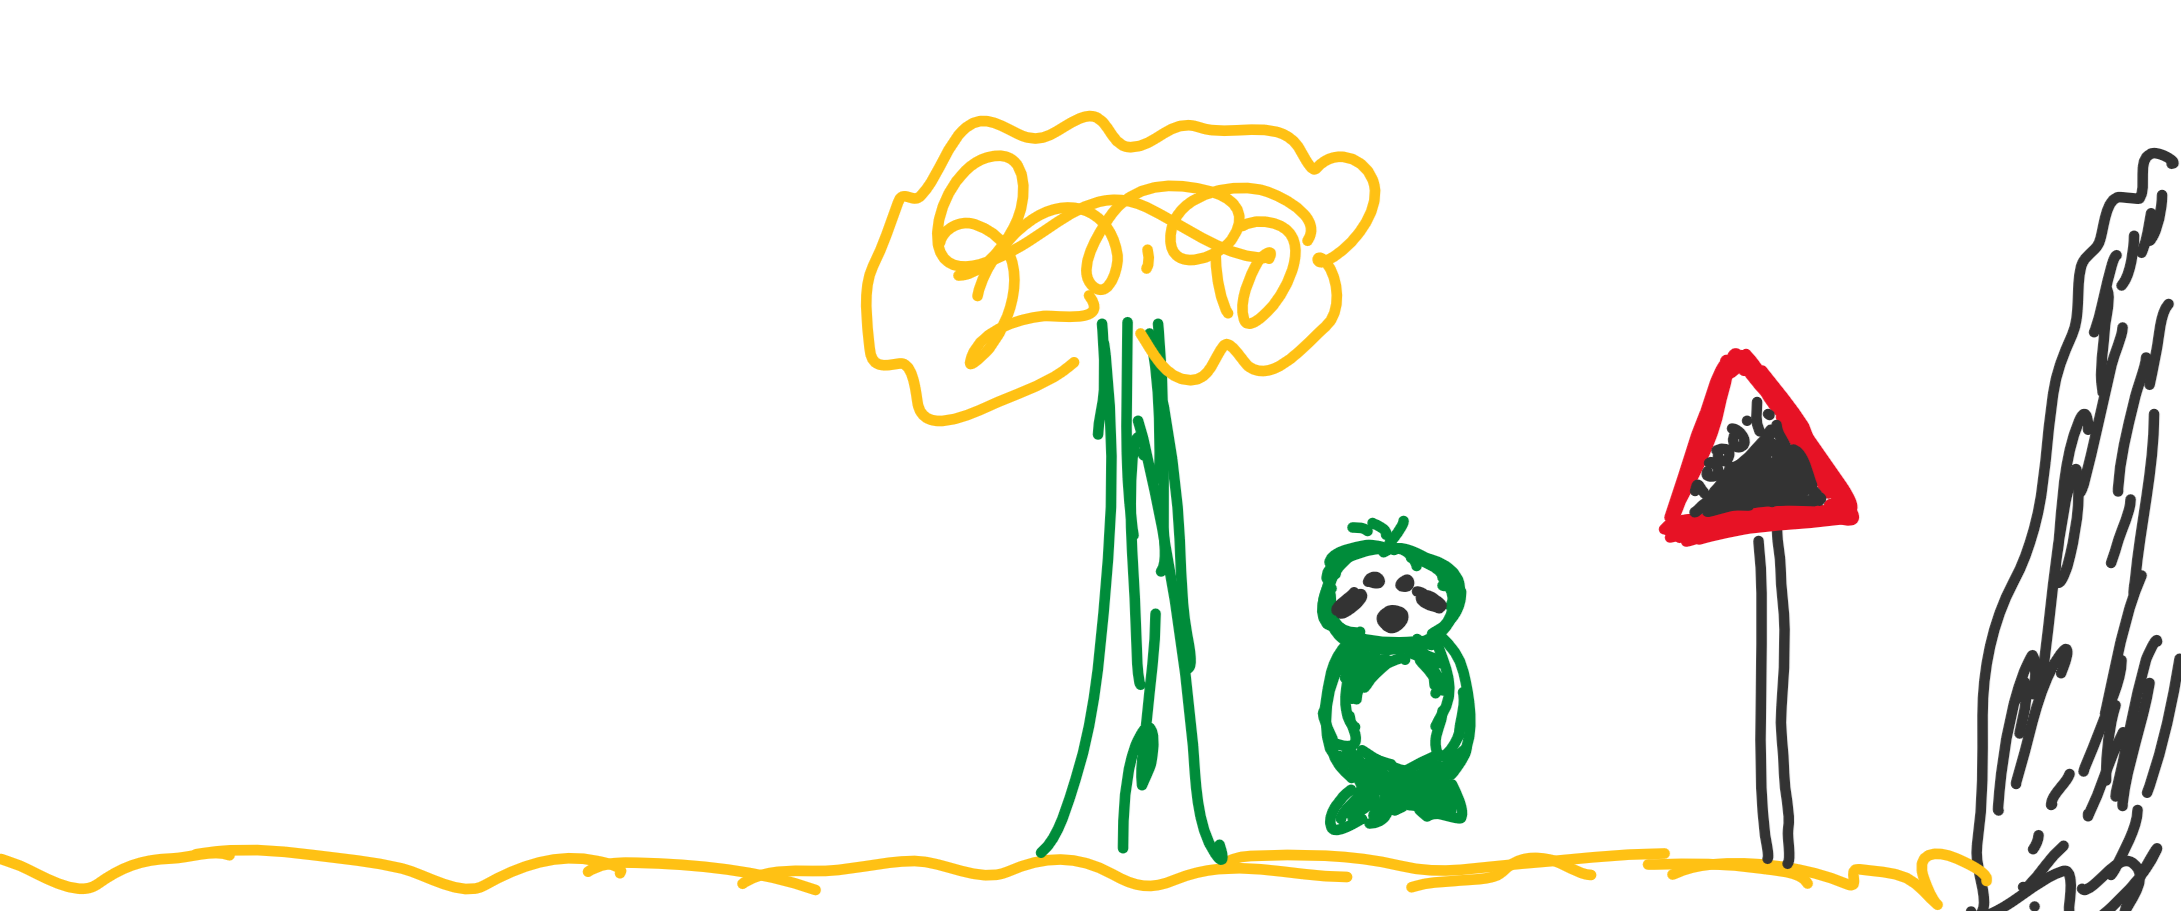
\includegraphics[height=5cm]{images/slope.png}
\end{center}

\begin{example}[ex:slope-always-equal]{}
    \parpic[r]{
        \begin{tikzpicture}
            \begin{axis}[defgrid, domain=0:5, y=1cm, x=1cm, xtick={1,...,5}, ytick={1,2,3},ymin=0,ymax=3,xmin=0,xmax=5, samples=2]
                \addplot[color=violet] expression{0.5*x};
                \addplot[mark=*, only marks, fill=violet] coordinates {(2,1)};
                \addplot[mark=*, only marks, fill=red] coordinates {(1,0.5)};
                \addplot[mark=*, only marks, fill=red] coordinates {(3,1.5)};
                \draw[very thick,dashed,-latex] (1,0.5) -- (2,0.5) -- (2,1);
                \draw[very thick,dashed,-latex] (2,1) -- (3,1) -- (3,1.5);
                \draw[very thick,dashed,-latex] (3,1.5) -- (4,1.5) -- (4,2);
            \end{axis}
        \end{tikzpicture}
    }
    Die rechts abgebildete Gerade ist nicht so steil wie die Gerade weiter oben auf dieser Seite. Wenn du vom violetten Punkt einen Schritt nach rechts gehst und schaust, wie stark die Gerade währenddessen angestiegen ist, dann siehst du, dass sie nur einen halben Schritt auf der $y$-Achse nach oben gekommen ist.
    
    \picskip{0}
    Dafür ist es aber vollkommen egal, ob du beim violetten Punkt anfängst oder beispielsweise bei einem der roten Punkte. Du machst immer dieselbe Beobachtung, wie stark die Gerade pro Schritt ansteigt -- denn sie ist ja überall gleich steil.
\end{example}

Während die Gerade in Beispiel \ref{ex:slope-always-equal} bei jedem Schritt nach rechts nur um $\frac{1}{2}$ nach oben gestiegen ist, hat die orangefarbene Gerade dabei immer $1$ Schritt in $y$-Richtung zurückgelegt. Dass die orangefarbene Gerade \emph{pro Schritt nach rechts} mehr Schritte nach oben zurücklegt, führt natürlich dazu, dass sie steiler ist.

Die Information, wie stark die Gerade \emph{pro Schritt nach rechts} ansteigt, genügt, um genau zu wissen, wie steil eine Gerade ist. Die Pfeile, die wir oben in die Bilder eingezeichnet haben, bilden zusammen mit dem Graphen ein Dreieck. Mithilfe eines solchen Dreiecks können wir die Steigung des Graphen bestimmen, indem wir schauen, wie hoch es ist. Deshalb heißen die Dreiecke, die wir eingezeichnet haben, \textbf{Steigungsdreiecke}. Unter der \textbf{Steigung} einer Gerade verstehen wir also die Höhe eines solchen Dreiecks mit der Breite $1$, weil dies genau wiederspiegelt, wie stark der Graph pro Schritt nach rechts ansteigt.

\begin{example}[ex:multiple-slope-examples]{}
    Die drei hier abgebildeten Geraden sind natürlich alle unterschiedlich steil: Die linke ist steiler als die mittlere und die rechte fällt sogar.
    \begin{multicols}{3}
        \begin{tikzpicture}
            \begin{axis}[defgrid, domain=0:3, y=0.75cm, x=1cm, xtick={1,...,3}, ytick={1,...,6},ymin=0,ymax=6,xmin=0,xmax=3, samples=2]
                \addplot[color=violet] expression{2*x};
                \addplot[mark=*, only marks, fill=violet] coordinates {(1,2)};
                \draw[very thick,dashed,-latex] (1,2) -- node[below] {$1$} (2,2) -- node[right] {$2$} (2,4);
            \end{axis}
        \end{tikzpicture}

        \begin{tikzpicture}
            \begin{axis}[defgrid, domain=0:3, y=0.75cm, x=1cm, xtick={1,...,3}, ytick={1,...,6},ymin=0,ymax=6,xmin=0,xmax=3, samples=2]
                \addplot[color=violet] expression{0.5*x+1.5};
                \addplot[mark=*, only marks, fill=violet] coordinates {(1,2)};
                \draw[very thick,dashed,-latex] (1,2) -- node[below] {$1$} (2,2) -- node[right] {$\frac{1}{2}$} (2,2.5);
            \end{axis}
        \end{tikzpicture}

        \begin{tikzpicture}
            \begin{axis}[defgrid, domain=0:3, y=0.75cm, x=1cm, xtick={1,...,3}, ytick={1,...,6},ymin=0,ymax=6,xmin=0,xmax=3, samples=2]
                \addplot[color=violet] expression{5-1.5*x};
                \addplot[mark=*, only marks, fill=violet] coordinates {(1,3.5)};
                \draw[very thick,dashed,-latex] (1,3.5) -- node[above] {$1$} (2,3.5) -- node[right] {$-\frac{3}{2}$} (2,2);
            \end{axis}
        \end{tikzpicture}
    \end{multicols}
    Mithilfe der eingezeichneten Steigungsdreiecke (alle haben eine Breite von $1$) lässt sich nun genau angeben, \emph{wie} steil die Geraden jeweils sind: Das Steigungsdreieck der ersten Gerade hat eine Höhe von $2$, also hat die linke Gerade eine Steigung von $2$. Die mittlere Gerade hat eine Steigung von $\frac{1}{2}$. Am besten siehst du das daran, dass du zwei Schritte nach rechts brauchst, um einen Schritt nach oben zu machen. Bei \emph{einem} Schritt nach rechts geht es also auch nur $\frac{1}{2}$ Schritt nach oben.

    Das Steigungsdreieck der rechten Gerade hat zwar eine Höhe von $1.5$ bzw. $\frac{3}{2}$, aber die Gerade hat eine negative Steigung von $-\frac{3}{2}$, denn der Pfeil zeigt nach unten.
\end{example}

Die Steigung jeder Geraden lässt sich also durch eine einzelne Zahl angeben. Nun liegt die Frage nahe, wie sich eine Gerade mit einer vorgegebenen Steigung durch eine Berechnungsvorschrift erzeugen lässt. 

\parpic[r]{
    \tikz{
        \begin{axis}[defgrid, domain=0:4, y=1cm, x=1cm, xtick={1,3.5}, ytick={0.6,2.1}, xticklabels={$x$,$x+1$}, yticklabels={$y$,$y+a$},ymin=0,ymax=3,xmin=0,xmax=4, samples=2]
            \addplot[color=violet] expression{0.6*x};
            \addplot[mark=*, only marks, fill=violet] coordinates {(3.5,2.1)};
            \addplot[mark=*, only marks, fill=violet] coordinates {(1,0.6)};
            \draw[very thick,dashed,-latex] (1,0.6) -- node[below] {$1$} (3.5,0.6);
            \draw[very thick,dashed,-latex] (3.5,0.6) -- node[right] {$a$} (3.5,2.1);
            \node[above] at (3.4,2.4) {\tiny $\coord{x+1}{y+a}$};
            \draw[-latex,violet,thick] (3.4,2.5) -- (3.5,2.15);
            \node[above] at (0.9,0.9) {\tiny $\coord{x}{y}$};
            \draw[-latex,violet,thick] (0.9,1) -- (1,0.65);
        \end{axis}
    }
}

Der Ausgangspunkt des Steigungsdreiecks hat jeweils eine bestimmte Koordinate $\coord{x}{y}$ und stellt die Zuordnungsregel $f(x)=y$ dar. Wenn wir jetzt auf einer Geraden mit der Steigung $a$ einen Schritt nach rechts gehen, dann erhalten wir einen Punkt, der die $x$-Koordinate $x+1$ hat (einen Schritt weiter rechts) und die $y$-Koordinate $y+a$ ($a$ Schritte weiter oben). Insgesamt ergibt das den Punkt $\coord{x+1}{y+a}$. Wir wissen nun also, dass
\[f(x)=y~\text{und}~f(x+1)=y+a\]
gelten muss. Wenn wir auf der rechten Seite $y$ durch $f(x)$ ersetzen, dann sehen wir, dass $f(x+1)=f(x)+a$ gelten muss. Weil eine Gerade immer gleich steil ist, legen wir die doppelte Distanz in $y$-Richtung zurück, wenn wir doppelt so weit nach rechts gehen -- bzw. die halbe Distanz, wenn wir halb so weit nach rechts gehen. Das bedeutet, dass wir nicht $a$, sondern $d\cdot a$ Schritte nach oben gehen, wenn wir $d$ Schritte statt einem nach rechts gehen. Es gilt also nicht nur $f(x+1)=f(x)+a$, sondern allgemeiner auch 
\[f(x+d)=f(x)+a\cdot d.\] Dies ist die zentrale Eigenschaft einer Gerade mit der Steigung $a$. Mit welchen Berechnungsvorschriften lässt sich das erreichen?

Bei linearen Gleichungen durfte auf jeder Seite ein Term der Art $ax+b$ stehen (mit Zahlen $a,b\in\Real$). Tatsächlich können wir mit einem solchen Term genau das erreichen, was wir wollen. Schauen wir uns einmal an, was passiert, wenn wir eine Funktion $f(x)=ax+b$ haben und $f(x+1)$ ausrechnen. Es gilt:
\[f(x+1)=a\cdot (x+1)+b=\colorobrace{ax+a}{a(x+1)}+b=\colorobrace{ax+b}{f(x)}+a=f(x)+a.\]
Hier steht also, dass der Funktionswert um $a$ größer wird, wenn wir um einen Schritt nach rechts gehen. Das ist genau die Eigenschaft, die eine Gerade mit der Steigung $a$ ausmacht und die wir bereits weiter oben formuliert haben.
% (streng genommen müssten wir noch prüfen, dass $f(x+d)=f(x)+a\cdot d$ auch für $d\neq 1$ gilt, aber das funktioniert mit der Rechnung
%\[f(x+d)=a\cdot (x+d)+b=\colorobrace{ax+a\cdot d}{a(x+d)}+b=\colorobrace{ax+b}{f(x)}+a\cdot d=f(x)+a\cdot d.\]
%genau auf dieselbe Weise). 
Eine Funktion $f$ mit der Berechnungsvorschrift $f(x)=ax+b$ ist also eine Gerade mit der Steigung $a$.

\begin{example}{}
    \parpic[r]{
        \begin{tabular}{cc}
            \toprule
            $x$ & $f(x)$\\
            \midrule
            1 & $2\cdot 1=2$\\
            2 & $2\cdot 2=4$\\
            3 & $2\cdot 3=6$\\
            4 & $2\cdot 4=8$\\
            $\vdots$ & $\vdots$\\
            $n$ & $2\cdot n=2n$\\
            \bottomrule
        \end{tabular}
    }
    Die linke Gerade aus Beispiel \ref{ex:multiple-slope-examples} hat eine Steigung von $2$. Sie gehört zur Funktion $f$ mit $f(x)=2x$. Pro Schritt nach rechts wird der Funktionswert der Funktion $f(x)=2x$ um $2$ größer. Der linke eingezeichnete Punkt stellt die Regel $f(1)=2$ dar.
    
    \picskip{4}
    Eine Einheit weiter rechts erhalten wir $f(2)=2\cdot 2=4$, also ist die Funktion tatsächlich um $2$ Einheiten gestiegen, während wir \emph{einen} Schritt nach rechts gemacht haben.
    \[f(1+1)=f(2)=2\cdot 2=4.\]
    In der rechts abgebildeten Tabelle siehst du weitere Funktionswerte, die wir ausgerechnet haben, um zu zeigen, dass die Funktion für jeden Schritt nach rechts einen um $2$ größeren Wert erhält.
\end{example}

\begin{definition}{Steigung einer Gerade}
    Es sei $f$ eine Funktion und $f(x)=ax+b$. Dann heißt $a$ die \textbf{Steigung} des Graphen von $f$.
\end{definition}

Wenn wir Funktionen haben, deren Graph eine Gerade ist, dann können wir die Steigung der Geraden also sofort aus der Berechnungsvorschrift ablesen, indem wir den Vorfaktor von $x$ anschauen (also das, was bisher das $a$ war). Beispielsweise hat der Graph von $f(x)=\frac{3}{2}x$ eine Steigung von $\frac{3}{2}$ (und ist natürlich eine Gerade). Damit wissen wir bereits deutlich mehr über den Graphen als vorher -- denn jetzt können wir einfach auf die Berechnungsvorschrift von $f$ schauen und wissen sofort, dass der Graph eine Gerade ist.

\parpic[r]{
    \tikz{
        \begin{axis}[defgrid, domain=0:3, y=0.75cm, x=1cm, xtick={1,...,3}, ytick={1,...,6},ymin=0,ymax=6,xmin=0,xmax=3, samples=2]
            \addplot[color=violet] expression{1.5*x+1};
            \addplot[color=orange] expression{1.5*x-0.5};
            \addplot[color=green!50!black] expression{1.5*x+2};
        \end{axis}
    }
}
Dennoch wissen wir noch nicht genau, wie der Graph von $f$ denn nun aussieht. Es gibt nämlich leider nicht nur eine Gerade mit der Steigung $\frac{3}{2}$. Die im rechten Bild dargestellten Geraden haben alle dieselbe Steigung. Ganz offensichtlich siehst du aber trotzdem drei unterschiedliche Geraden. Sie sind alle parallel zu einander, aber um eine von ihnen zu beschreiben, benötigen wir neben der Steigung noch eine weitere Information, die beschreibt, wie weit oben oder unten die Gerade liegt. 

Du siehst, dass alle Geraden die $y$-Achse an einem anderen Punkt schneiden: Die grüne Gerade bei $2$, die violette bei $1$ und die orangefarbene irgendwo im negativen Bereich. Wüsstest du über eine Gerade zusätzlich zur Steigung noch, wo sie die $y$-Achse schneidet, dann könntest du auch sagen, wie weit oben die Gerade im Koordinatensystem liegt. Diese Information liefert der \emph{Achsenabschnitt}, den du bereits im Kapitel über \emph{Funktionen} kennengelernt hast.

Aus dem Kapitel über \emph{Funktionen} weißt du bereits, dass der Achsenabschnitt einer Funktion die Zahl ist, die du erhältst, wenn du $f(0)$ ausrechnest. Für $f(x)=ax+b$ können wir $f(0)$ leicht ausrechnen. Es gilt
\[f(0)=a\cdot 0+b=b.\]
Die Funktion $f(x)=ax+b$ hat also den Achsenabschnitt $b$. Damit wissen wir jetzt genau, wie der Graph einer Funktion aussieht, die die Berechnungsvorschrift $f(x)=ax+b$ hat:
\begin{itemize}
    \item der Graph ist eine Gerade mit der Steigung $a$
    \item der Graph hat den Achsenabschnitt $b$
\end{itemize}

\begin{theorem}{Geradengleichungen}
    Der Graph einer Funktion $f(x)=ax+b$ ist eine Gerade mit der Steigung $a$ und dem Achsenabschnitt $b$.
\end{theorem}

Grundsätzlich kannst du dir merken, dass du zum Beschreiben einer Gerade immer zwei Informationen benötigst: Die Richtung und die Information, wie weit oben die Gerade liegt. Diese Informationen kannst du durch die Steigung und den Achsenabschnitt bekommen.

\begin{example}{}
    \parpic[r]{
        \begin{tikzpicture}
            \begin{axis}[defgrid, domain=0:4, y=0.5cm, x=1cm, xtick={1,...,4}, ytick={-5,...,7},ymin=-5,ymax=7,xmin=0,xmax=4, samples=2]
                \addplot[color=violet] expression{3*x-5};
                \addplot[mark=*, only marks, fill=violet] coordinates {(0,-5)};
                \addplot[mark=*, only marks, fill=violet] coordinates {(1,-2)};
            \end{axis}
        \end{tikzpicture}
    }
    Zu Beginn dieses Abschnitts haben wir die Frage gestellt, wie der Graph der Funktion 
    \[f(x)=\tikzmarknode{slope3x5}{3}x\tikzmarknode{axis3x5}{-5}\] 
    aussieht. Bereits vor dem Lesen dieses Kapitels wusstest du, dass er die $y$-Achse im Punkt $\coord{0}{-5}$ schneidet, also den \textcolor{violet}{Achsenabschnitt} $-5$ hat, denn es gilt $f(0)=-5$.
    \tikz[overlay, remember picture]{
        \draw[maincolor] ($(slope3x5) + (-0.75ex,-1ex)$) -- ++ (1.5ex, 0) -- ++ (0,2ex) -- ++ (-1.5ex,0) -- cycle;
        \draw[violet] ($(axis3x5) + (-1.4ex,-1ex)$) -- ++ (2.8ex, 0) -- ++ (0,2ex) -- ++ (-2.8ex,0) -- cycle;
    }
    Jetzt bist du sogar in der Lage, den Graphen vollständig zu zeichnen. Es handelt sich nämlich um eine Gerade durch den Punkt $\coord{0}{-5}$, die eine \textcolor{maincolor}{Steigung} von $3$ hat, also pro Schritt nach rechts drei Schritte nach oben steigt.

    \picskip{1}
    Mithilfe dieser beiden Informationen (also Steigung und Achsenabschnitt) ist eindeutig festgelegt, dass die Gerade wie rechts abgebildet aussehen muss. Du kannst sie zeichnen, indem du beim Punkt auf der $y$-Achse beginnst, den du als Achsenabschnitt berechnet hast (linker violetter Punkt). Anschließend zeichnest du einen Punkt einen Schritt weiter rechts ein, der $3$ Schritte weiter oben liegt als der erste Punkt (denn $3$ ist die Steigung). Dann zeichnest du eine Gerade durch die beiden Punkte und erhältst den Graphen der Funktion $f$.
\end{example}

Möchtest du den Graphen einer Funktion mit der Berechnungsvorschrift $f(x)=ax+b$ zeichnen, dann brauchst du eigentlich immer zwei Punkte, die du verbinden kannst, um eine Gerade zu zeichnen. Die Punkte kannst du einfach berechnen, indem du zwei verschiedene Werte für $x$ in die Funktion einsetzt und jeweils $f(x)$ berechnest. Dadurch erhältst du die Koordinaten von zwei Punkten auf dem Graphen und kannst ihn zeichnen.

\begin{nutshell}{Geradengleichungen}
    \parpic[r]{
        \begin{tikzpicture}
            \begin{axis}[defgrid, domain=0:3, y=0.75cm, x=1cm, xtick={1,...,3}, ytick={1,...,4},ymin=0,ymax=4,xmin=0,xmax=3, samples=2]
                \addplot[color=violet] expression{0.8*x+1.2};
                \addplot[mark=*, only marks, fill=violet] coordinates {(1,2)};
                \draw[very thick,dashed,-latex] (1,2) -- node[below] {$1$} (2,2) -- node[right] {$a$} (2,2.8);
            \end{axis}
        \end{tikzpicture}
    }
    Der Graph mancher Funktionen hat die Form einer Geraden. Bei solchen Funktionen lässt sich ein enger Zusammenhang zwischen ihrer Berechnungsvorschrift und dem Aussehen ihres Graphen feststellen. Eine Gerade im Koordinatensystem kann durch ihre \textbf{Steigung} (also die Schritte der Gerade nach oben \emph{pro Schritt nach rechts}) und ihren \textbf{Achsenabschnitt} beschrieben werden.
    
    \picskip{1}
    Um die Steigung einer Gerade zu bestimmen, kann ein \textbf{Steigungsdreieck} verwendet werden. Dafür wird ein Punkt auf der Geraden gewählt, von dem aus ein Dreieck mit einer Breite von $1$ nach rechts gezeichnet wird. Die Steigung der Geraden entspricht dann der Höhe des Dreiecks. Die Berechnungsvorschrift, die zu einer Geraden mit der Steigung $a$ und dem Achsenabschnitt $b$ gehört, ist
    \[f(x)=ax+b.\]
\end{nutshell}

\end{document}
